%%%%%%%%%%%%%%%%%%%%%%%%%%%%%%%%%%%%%%%%%%%%%%%%%%%%%%%%%
%%%%%%%%%%%%%%%%%%% author:hijeffery %%%%%%%%%%%%%%%%%%%%
%%%%%%%%%%%%%%%%%%% part:14.0-14.6   %%%%%%%%%%%%%%%%%%%%
%%%%%%%%%%%%%%%%%%%%%%%%%%%%%%%%%%%%%%%%%%%%%%%%%%%%%%%%%

\chapter{自编码器}
\label{chap:14}

\emph{自编码器}是神经网络的一种,用以训练来实现将输入复制到输出的目的。在其内部,有一个用编码表示输入的隐层$h$。自编码器可以看作由两部分组成:编码函数$h = f(x)$ 和进行信号重建的解码函数$r = g(h)$。 具体结构如图\ref{fig:14.1}所示。如果自编码器学到的结果仅仅是处处将$g(f(x)) = x$,则其没有起到任何作用。相反,自编码器被设计成了不能够完美的复制输入到输出的工作方式。通常他们被限定在只能够近似的复制,并且只复制能够与训练数据相像的输入。鉴于模型被强制执行输入的某些部分应当被复制,所以通常来讲,自编码器能够学习到数据的有用的特性。
\begin{figure}[htbp] %  figure placement: here, top, bottom, or page
   \centering
   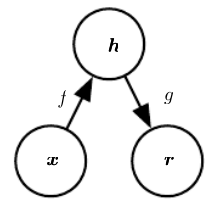
\includegraphics[width=1in]{fig/chap14/14_1.png} 
   \caption{自编码器的基本结构,将输入信号$x$通过一个内部表征或者编码$h$ 映射到输出(也叫重建) $r$。 自编码器有两个子部分:编码器(将$x$映射到$h$)与解码器(将$h$映射到$r$)。}
   \label{fig:14.1}
\end{figure}

现代自编码器已经从执行特定的函数映射扩展到了执行随机映射$p_{encoder}(h|x)$ 和 $p_{decoder}(x|h)$。

自编码器的思想已经在神经网络研究领域存在了几十年。传统上来讲,自编码器是用来执行数据降维与特征学习的。近来,自编码器与隐变量模型的联系使得自编码器成为生成模型的研究前沿,详情见本书第\ref{chap:20}章介绍。自编码器可以视为前馈网络的一种特殊形式,并且可以用与其相同的方式进行训练,如以子集沿着反向传播计算的梯度下降方向求解。同一般的前馈网络不同的是,自编码器也可以用\emph{再循环}的方式进行训练,即对比原始输入的网络相应与重建信号作为输入的网络相应的差别。再循环技术被视为比反向传播算法更为接近生物特性的方法,但是其很少被出现在其他机器学习应用中。

\section{不完备自编码器}
\label{sec:14.1}
将输入复制到输出听起来似乎无特别作用,但其实我们也不关心解码器的输出。事实上,我们期望通过训练自编码器实现复制输入的任务能够产生有实用意义的$h$。

一个从自编码器获取有效的特征的方法是将$h$限定到一个比$x$更低的维度上。特征维度比输入维度低的自编码器是\emph{不完备}的。学习一个不完备的特征迫使自编码器捕获到训练数据中的最为突出的特征信息。

学习过程可以简单的表述为最小化一个随时函数的形式:
\begin{equation}
	L(x,g(f(x)))
\end{equation}
其中,损失函数 $L$ 通过如最小化均方误差等限定$g(f(x))$ 与 $x$ 尽量相近。 

当解码器是线性函数,并且$L$ 是均方误差时,不完备自编码器学习到的生成子空间与PCA一致。此时,被用来执行复制任务的自编码器事实上附加学到了训练数据的主子空间。

因此,具有非线性编码函数$f$和非线性解码函数$g$的自编码器可以学习到更强有力的非线性泛化PCA。遗憾的是,如果编码与解码部分被给予太强能力的化,自编码器仍然仅仅完成复制输入到输出的功能而忽略了抽取数据分布等有效信息的能力。理论上说,我们可以设想一个只有一维编码的自编码器,其编码器具有强大的能力将每一个训练数据$x^{(i)}$表示成编码$i$。此外,解码器能够学习并将每一个整型值映射回特定的训练数值上。这种特殊情形在现实中不会出现,但其足够说明,一个被训练用来进行数据复制的自编码器,如果被赋予了过与强大的能力,并不会学习到任何与用的信息。

\section{正则化自编码器}
\label{sec:14.2}
编码维数比输入维数低的自编码器能够学习到数据分布的最为显著的信息。我们也提到,如果编码与解码部分被赋予了太强的能力,会导致自编码器学习不到任何有用的东西。

相似的问题也会发生在编码维数同输入维数相同的自编码器中,以及隐层编码维数比输入数据维数大的\emph{过完备}自编码器中。在这种情况时,甚至线性的编码器与解码器也会产生直接复制输入数据到输出数据而不获取任何数据分布有效信息的问题。

理想来说,我们只要根据待建模分布的复杂度选取编码的维数以及编码器解码器的容量,我们就可以成功的训练任何结构的自编码器。正则化自编码器就提供了这种功能。正则化自编码器不是通过控制编码器解码器的层数与编码长度来达到限定模型容量的目的,而是通过损失函数来促使模型具有复制输入到输出以外的特性的。这些特性包括描述特征的稀疏度,缩小特征的偏导数以及对于噪声和数据确实的鲁棒性等。正则化自编码器可以是非线性的或者过完备的,但是,即便有足够容量可以取巧只学习简单的复制函数,其仍可以学习到数据分布的一些有用的东西。

除了本处列举的几个可以被很自然的理解为正则化自编码器的方法之外,几乎任何有隐变量以及推理过程(从给定输入推算隐变量表示)的生成模型都可以被视为一种具有特殊形式的自编码器。有两种同自编码器有此种高度关联的生成模型如变分自编码器和随机生成网络,他们都是Helmholtz机的子类。这些模型会自然的学习高容量,过完备的编码方式,并且不需要归一化处理才能使这些编码具有实用性。这些编码之所以有效,是因为模型是被训练来近似最大化训练数据的概率分布,而不是去执行复制输入输出的操作。

\subsection{稀疏自编码器}
\label{sec:14.2.1}
稀疏自编码器是在自编码器的基础上,简单的引入稀疏惩罚项$\Omega(h)$加到编码层上,并同重建误差项一起训练:
\begin{equation}
L(x,g(f(x))) + \Omega(h) 
\end{equation}
其中,$g(h)$ 是解码器的输出,并且通常编码器的输出为$h = f(x)$。

稀稀疏自编码器通常被用于其他任务中,如分类。稀疏泛化的自编码器必须能够对其针对的训练数据的特定统计特性做出响应,而不能是简单的复制操作。此时,训练执行复制任务,并且有一定的稀疏惩罚项能够得到具有附加特征表示能力的模型。

我们可以把惩罚项$\Omega(h)$ 简单的看作添加到前馈网络上的正则项,该网络主要是实现复制输入到输出的任务(非监督学习目标函数),或者根据这些稀疏特征执行一些有监督的任务(监督学习目标函数)。
同其他正则项如权值衰减等不同,改该正则项并没有直观的贝叶斯解释。如\ref{sec:5.6.1}中所描述,包含权值衰减和其他正则化惩罚项的训练过程可以被视为贝叶斯推断的最大后验近似,其中加入的正则惩罚项可以视为参数模型的先验概率。在这个角度,最大化的最大似然同最大化$p(\theta|x)$相关,有等效于最大化$log p(x|\theta) + log p(\theta)$。$log p(x|\theta)$是常规的数据对数似然项,对数先验项$log p(\theta)$包含对于$\theta$的某些特定值的偏好。这部分内容在第\ref{sec:5.6}节中有介绍。正则化自编码器则不赞同这种解释,因为正则项本身依赖于数据,因此语义上来讲,其定义并不是严格的先验。

与其将稀疏惩罚项视为复制任务的正则项,我们不妨将整个稀疏自编码框架看过是有隐变量的生成模型最大似然训练。假设我们有一个模型,其观测变量为$\bm{x}$隐变量为$\bm{h}$,并且其联合概率分布为$p_{model}(\bm{x},\bm{h}) = p_{model}(\bm{x}|\bm{h})$。我们定义$p_{model}(\bm{h})$为模型对于隐变量的先验概率,表示模型在观察变量$\bm{x}$前的置信度。同我们之前使用“先验”这个词有些不同,这里是指,在我们观察到训练数据之前,$p(\bm{\theta})$ 代表了我们对于模型参数的置信度。其对数似然可以分解为
\begin{equation}
	log p_{model}(\bm{x}) = log \sum_{\bm{h}}p_{model}(\bm{h},\bm{x})
\end{equation}
自编码器可以视为用$\bm{h}$的一个最相似的点对上述求和的近似。这同稀疏表示生成模型(\ref{sec:13.4}节)很像,但$\bm{h}$是参数化编码器的输出而不是推测最相似$\bm{sh}$的优化结果。从这个角度,给定$\bm{h}$后,须最大化
\begin{equation}
	log p_{model}(\bm{h},\bm{x}) = log p_{model}(\bm{h}) + log p_{model}(\bm{x}|\bm{h})
\end{equation}
其中,$log p_{model}(\bm{h})$ 可以是稀疏诱导项。比如,拉普拉斯先验,
\begin{equation}
	p_{model}(h_i) = \frac{\lambda}{2}e^{- \lambda |h_i|},
\end{equation}
对应着一个绝对值的稀疏惩罚项。将对数先验表示为绝对值惩罚项,则
\begin{equation}
	\Omega(\bm{h}) = \lambda \sum_i | h_i |
\end{equation}
\begin{equation}
	-log p_{model}(\bm(h)) = \sum_i (\lambda|h_i| - log \frac{\lambda}{2}) = \Omega(\bm{h}) + const
\end{equation}
其中,常数项只与$\lambda$有关,与$\bm{h}$无关。我们通常将$\lambda$视为超参数并忽略常数项,因为其对于参数学习没有影响。其他的先验函数如student-t分布,同样可以引入稀疏性。因为稀疏性是在用$p_{model}(\bm{h})$近似最大似然估计学习的过程中引入的,因此,从这个角度来看,稀疏惩罚项根本不能算作正则项。它仅仅是一系列模型隐变量分布的结果。这个思路给自编码器训练了一个不同的动机:其是训练生成模型的一个近似方法。同时,也给为什么自编码器学习到的特征有用提供了新的原因:他们描述了能够解释输入的隐变量。

稀疏自编码器的早期工作介绍了多种形式的稀疏,并提出了稀疏惩罚项同$log Z$之间的关系,$log Z$是在用最大似然估计无向图模型$p(x) = \frac{1}{Z}\hat{p}(x)$时产生的。其基本思路是,最小化$log Z$能够防止图模型在各处产生很高的概率,而对自编码器引入稀疏性能够防止在任意地方产生极低的重建误差。这种情况下,二者的联系存在于一个比较直观的普通机制理解层面上而不是仅仅有数学联系。在有向图模型$p_{model}(\bm{h}p_{model}(\bm{x}|\bm{h})$中,与稀疏项有关的$log p_{model}(\bm{h})$则具有更好的数学直观解释。

Glorot等人给出了一个实现稀疏(降噪)自编码器隐层编码$\bm{h}$中\emph{绝对零值}的方法。其思路是用ReLU来生成编码层。有了能够使描述逼近零值的先验(比如绝对值惩罚项),我们可以用间接的手段来控制特征表示中的零值的平均个数。

\subsection{降噪自编码器}
除了给损失函数添加惩罚项$\Omega$外,我们还可以通过改变损失函数项来实现训练自编码器学习有效信息的方法。

传统的自编码器的损失函数为
\begin{equation}
L(x,g(f(x)))
\end{equation}
其中,$L$是限定$g(f(x))$同 $x$相似度的损失函数,如对比二者的$L^2$ 范数损失。这使得$g\circ f$ 如果有能力的化就会学习到一个复制函数。

而\emph{降噪自编码器}则是最小化
\begin{equation}
L(x,g(f(\hat{x})))
\end{equation}
其中,$\hat{x}$是$x$ 被某种噪声干扰后的数据。降噪自编码器必须设法处理这种干扰而不是仅仅复制输入数据。

降噪训练的过程迫使$f$和$g$去学习潜在的$p_{data}(x)$的结构。降噪自编码器再次印证了在最小化重建误差的过程中,会有很多有用的性质作为副产品出现。
他们也可以作为过完备、高容量模型可以用来作为自编码器的例子,只要这些模型能够加入防止其学习到恒等函数的设计即可。      
降噪自编码器在第\ref{sec:14.5}节有更为详细的介绍。

\subsection{梯度惩罚正则化}
另一个正则化自编码器的方法是通过借用稀疏自编码器中的惩罚项$\Omega$, 
\begin{equation}
L(x,g(f(x))) + \Omega(h,x),
\end{equation}
但是,此处用了一个不同形式的$\Omega$
\begin{equation}
\Omega(h,x) = \lambda \sum_i \| \nabla_x h_i\|^2.
\end{equation}
这使得模型能够学到一个当$x$发生轻微变化的时候不会改变太多的函数。由于这个惩罚项仅仅作用于训练数据,其迫使自编码器能够捕获到训练数据的分布信息。

此种方式泛化的自编码器被成为\emph{收缩自编码器}。这种方法同降噪自编码器,流行学习以及概率模型具有很强的理论联系。更多的细节参看\ref{sec:14.7}节。

\section{表征能力,层级及深度}
\label{sec:14.3}
自编码器的训练通常只包含一层编码器和一层解码器。然而,这不是绝对的。事实上,用多层编码器和解码器能够提供非常多的好处。

我们可以回想第\ref{sec:6.4.1}节所述,用多层网络对于前馈型神经网络有很多的好处。因为自编码器是前馈型神经网络,这些优势也同样适用。此外,自编码器的编码器和解码器本身也都是前馈网络,所以这两部分都可以单独从网络深度获益。

网络深度的不平凡之处在于通用近似理论确保了对于有至少一层隐藏层的前馈神经网络,只要其具有足够的隐藏节点,就能够以任意精度近似任何函数(在一个很广的分类限定内)。这意味着具有一个隐藏层的自编码器就可以在数据域内足够好的近似恒等函数。但是,从输入到特征编码的映射是浅层的。这意味着我们无法满足随意的限定,如编码必须是稀疏的等。一个深度的自编码器,在编码器内部有至少一层隐藏层的情况下,如果有足够的隐藏节点,就可以任意好的近似从输入到编码的任意映射函数。

网络深度可以以指数级的优势降低某些方程的计算复杂度。网络深度也可以以指数级降低训练某些函数所需要的训练样本的数量。请看参看\ref{sec:6.4.1}获取更多的网络深度对于前馈型网络的优势的信息。

实验效果上来说,深度自编码器比传统的浅层或者线性自编码器具有更好的特征压缩性能。

训练深度自编码网络的一个常见手法是逐层训练一个堆叠的浅层自编码器,所以,即便我们的最终目标是训练一个深度自编码器,我们其实常常还是会遇到浅层自编码器。

\section{随机编码与解码}
\label{sec:14.4}
自编码器就是前馈型神经网络的一种。传统前馈神经网络的损失函数和输出单元都可以用到自编码器中。

如第\ref{sec:6.2.2.4}节所描述,设计前馈神经网络输出单元与损失函数的一个常用的策略就是定义一个输出分布$p(y| x)$ 并且最小化其负指数似然函数$-log p(y|x)$。在这种情况下,$y$是目标向量,如分类的类别标记。

在自编码器的情况下,$\bm{x}$既是输入也是输出。但是,我们仍然可以使用以前的学习机制。给定一个隐层编码$\bm{h}$,我们可以把解码器视为条件概率分布$p_{decoder}(\bm{x}|\bm{h})$。我们可以通过最小化$-log p_{decoder}(\bm{x}|\bm{h})$来训练自编码器损失函数的具体形式会根据$p_{decoder}$而发生改变。同传统前馈神经网络一样,如果$\bm{x}$是实数值的话,我们通常用线性输出单元来参数化高斯分布的均值。此时,付对数似然等效于最小均方误差。相似的,二进制$\bm{x}$值对应与伯努利分布,其参数由sigmoid函数给出;离散$\bm{x}$值对应于softmax分布等等。一般来讲,输出被视为独立于隐层单元$\bm{h}$,如此,概率分布的计算相对容易求解。但是有些方法如混合密度输出允许借助协方差来连续建模。

为了比前面介绍的前馈神经网络有一个更根本的转变,我们可以把\emph{编码函数}$f(\bm{x})$表示为\emph{编码分布}$p_{encoder}(\bm{h}|\bm{x})$,如图\ref{fig:14.2}所示。
\begin{figure}[htbp] %  figure placement: here, top, bottom, or page
   \centering
   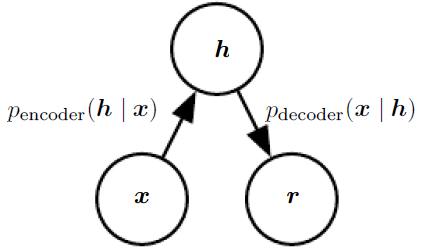
\includegraphics[width=2in]{fig/chap14/14_2.png} 
   \caption{随机自编码器结构图。其中编码器与解码器都不是简单的函数而是包含了一些噪声,这意味着他们的输出可以看作是从要给概率分布中抽样获得的,编码的分布为$p_{encoder(\bm{h}|\bm{x})}$,解码的分布为$p_{decoder}(\bm{x}|\bm{h})$。}
   \label{fig:14.2}
\end{figure}

任何隐变量模型$p_{model}(h,x)$都可以用来定义随机编码器
\begin{equation}
	p_{encoder}(h|x) = p_{model}(h|x)
\end{equation}
和随机解码器
\begin{equation}
	p_{decoder}(x|h) = p_{model}(x|h)
\end{equation}
通常来讲,编码器和解码器并不一定是同联合概率分布$p_{model}(x,h)$吻合的条件概率分布。Alain指出作为降噪自编码训练编码器和解码器能够使他们渐进兼容(在有足够容量和样本的情况下)。

\section{降噪自编码器}
\label{sec:14.5}
降噪自编码器是在给定的输入包含噪声的情况下训练以预测其未被干扰的输入的自编码器。

降噪自编码器额训练过程在图\ref{fig:14.3}中给出。我们介绍加噪处理$C(\hat{x}|x)$,其代表在给出训练样本$x$时的$\hat{x}$的条件概率分布。自编码器从训练样本对$(x,\hat{x})$中学习到\emph{重建分布}$p_{reconstruction}(x|\hat{x})$,过程如下:

1. 从训练样本中抽取一个样本$x$。

2. 从分布$C(\hat{x}|x)$中抽取带有噪声的样本$\hat{x}$。

3. 将$(x,\hat{x})$作为训练样本去预测自编码器的重建分布$p_{reconstruction}(x|\hat{x}) = p_{decoder}(x|h)$,其中,$\bm{h}$是编码器$f(\hat{x})$的输出,$p_{decoder}$一般是由解码器$g(\bm{h})$给出。

一般来讲,我们可以对负对数似然$-log p_{decoder}(x|h)$做基于梯度的近似最小化(如小批次梯度下降)。只要编码器是确定性的,降噪自编码器就是前馈神经网络,并且可以用其他前馈网络的训练方法进行训练。
\begin{figure}[htbp] %  figure placement: here, top, bottom, or page
   \centering
   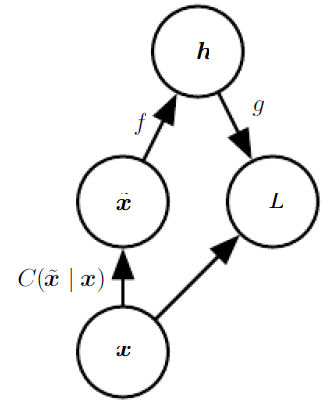
\includegraphics[width=2in]{fig/chap14/14_3.png} 
   \caption{降噪自编码器的损失计算图,即训练其使得能够从带噪声的样本$\hat{x}$中恢复出干净的样本$x$来。训练是通过最小化损失$L = -log p_{decoder}(x|h = f(\hat{x}))$得到的,其中$\hat{x}$是从加噪函数$C(\hat{x}|x)$得到的含有噪声版本的$x$。通常$p_{decoder}$是一个因子分布,其参数均值由前向网络$g$给出。}
   \label{fig:14.3}
\end{figure}

我们可以把降噪自编码器看作是针对下面期望的随机梯度下降:
\begin{equation}
 -\mathbb{E}_{x\sim \hat{p}_{data}(x)}\mathbb{E}_{\hat{x} \sim C(\hat{x}|x)}log p_{decoder}(x| h = f(\hat{x}))
\end{equation}
其中,$\hat{p}_{data}(x)$是训练样本分布。

\subsection{估算评分}
\label{sec:14.5.1}
评分估计是最大似然估计的一种替代方法。它能够通过促使模型在每一个样本点上同数据分布有一样的评分来给出概率分布的一个一致的估计值。此处,这个评分是一个特别的梯度域:
\begin{equation}
	\nabla_x log p(\bm{x})
\end{equation}
评分匹配在第\ref{sec:18.4}节中有更为细致的讲解。就当前对自编码器的讨论来讲,了解学习梯度域$log p_{data}$ 是学习$p_{data}$结构的一种方法就足够了。

降噪自编码的一个非常重要的性质就是他们的训练准则(用条件高斯$p(\bm{x}|\bm{h})$)使得自编码器学习到了一个计算数据分布评分的向量域$(g(f(x)) - x)$。请参考图\ref{fig:14.4}。
\begin{figure}[htbp] %  figure placement: here, top, bottom, or page
   \centering
   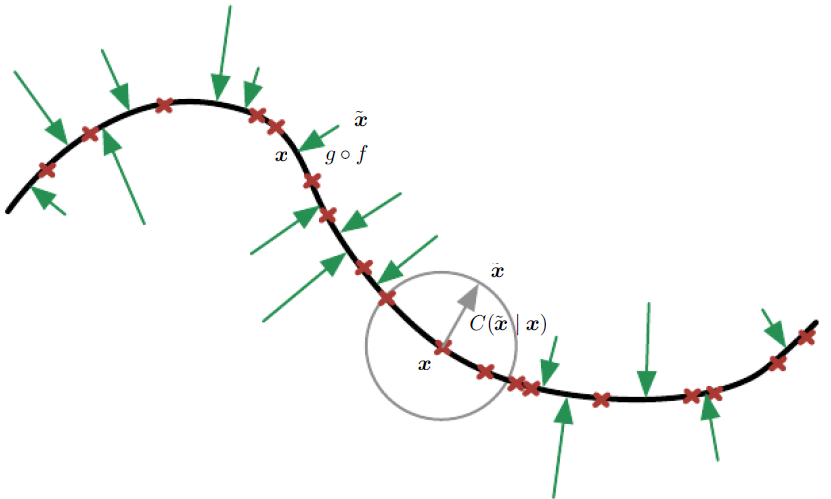
\includegraphics[width=4.5in]{fig/chap14/14_4.png} 
   \caption{降噪自编码器被训练用以将含噪数据$\hat{\bm{x}}$映射回原始数据$\bm{x}$。原始数据用红色X号表示,其处于黑色实线表示的一维流面上。加噪函数$C(\bm{\hat{x}},\bm{x})$用灰色圆圈表示其各向同性。灰色箭头表示了样本是如和从流面被引入噪声映射到别处的。当降噪自编码器被训练来降低均方误差$\|g(f(\hat{x})) -x \|^2$时,重建函数$g(f(\hat{x}))$计算了期望$\mathbb{E}_{x,\hat{x} \sim p_{data} C(\bm{\hat{x}}, \bm{x})}[\bm{x}|\bm{\hat{x}}]$。向量$g(f(\hat{\bm{x}})) - \hat{\bm{x}}$指向了流面上最近的点,这是因为$g(f(\hat{\bm{x}}))$估算的可能产生噪点$\bm{\hat{x}}$的纯净数据$\bm{x}$的重心。因此自编码器学习到了一个向量空间$g(f(\hat{\bm{x}})) - \bm{x}$,图中绿线所示。这个向量域用一系列乘数因子计算评分$\nabla x \log p_{data}(\bm{x})$,这些因子是重建均方误差的根值平均数。}
   \label{fig:14.4}
\end{figure}

用高斯噪声和均方差作为重建损失来训练一个特定的降噪自编码器(隐层为sigmoid单元,重建为线性单元)等效于训练一种特定的具有高斯可观察单元的称为RBM的无向图模型。这种模型将会在第\ref{SEC:20.5.1}节进行详细介绍;此处仅需知道他是一种能够提供明确函数$p_{model}(\bm{x};\bm{\theta})$的模型即可。当RBM被用\emph{降噪评分匹配}来进行训练的时候,其学习算法等同于和它对应的自编码器的降噪训练。给定特定的噪声值,泛化评分匹配并不是一个一致的估算;它其实恢复了一个模糊化的分布。但是,如果噪声水平接近于零,并且训练样本趋近于无穷,此时一致性又得到了恢复。降噪评分匹配在第\ref{sec:18.5}节有详细讨论。

RBM同自编码器还有其他的联系。评分匹配应用到RBM上产生的损失函数等同于重建误差加上一个同收缩自编码中的收缩项相似的正则化项。Bengio等人指出自编码器的导数为RBM的contrastive divergance计算提供了近似。

对于连续值$\bm{x}$,包含高斯噪声和重建分布的降噪标准为常规编码器和解码器的参数化评分计算提供了依据。这意味着生成编码-解码结构通过训练后可以被用来计算评分,训练用的均方误差标准为
\begin{equation}
	\|g(f(\bm{\hat{x}})) - \bm{x}\|^2
\end{equation}
以及噪声
\begin{equation}
	C(\hat{x} = \bm{\hat{x}} | \bm{x}) = \mathcal{N}(\bm{\hat{x}}; \mu = \bm{x}, \Sigma = \sigma^2I)
\end{equation}
其中,$\sigma^2$为噪声方差。关于具体如何运作,请参考图\ref{fig:14.5}。
\begin{figure}[htbp] %  figure placement: here, top, bottom, or page
   \centering
   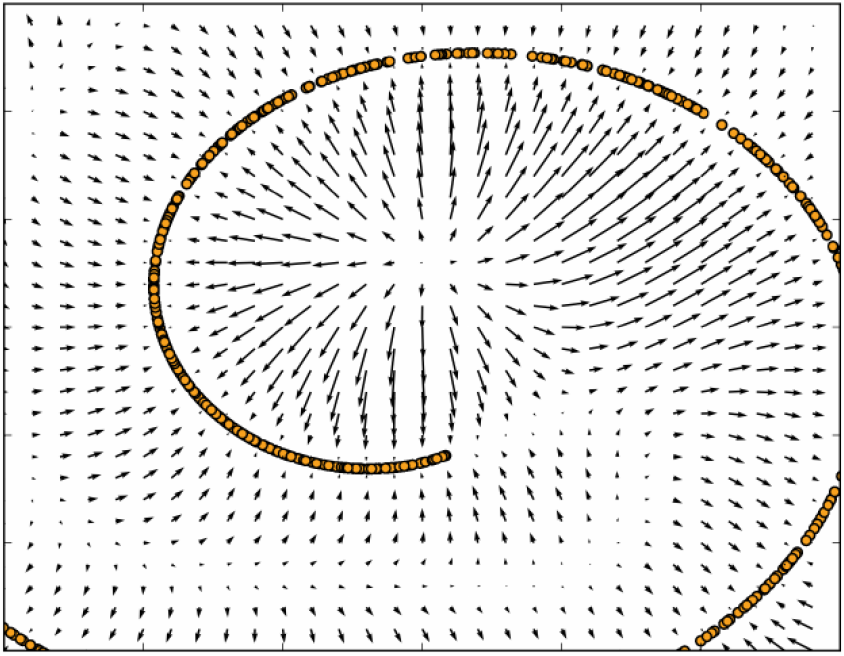
\includegraphics[width=4.5in]{fig/chap14/14_5.png} 
   \caption{降噪自编码器学习到的二维空间中的一维曲面流面附近的向量域。每一个箭头都与重建向量减去输入向量的值成一定比例并且箭头指向预测到的概率分布的较高概率值。向量域在估算的密度函数的极大值(在数据流面上)与极小值处取值为零。例如,螺旋的臂构成了相互连接的有局部极大值的一维流面。局部极小值在两个臂之间的区域的中间位置。当重建误差的模(以箭头的长度表示)较大的时候,意味着沿着箭头的方向移动的话概率值可以得到很大的提升,反之亦然。自编码器将这些低概率的点映射为高概率的重建值。在概率取得极大值的地方,箭头缩短,因为此时的重建值更加精确。}
   \label{fig:14.5}
\end{figure}

通常来讲,并没有任何保证说重建$g(f(x))$ 减去输入$\bm{x}$对应于任何方程的导数,更别提评分了。如此可以解释为什么早期的结果只能应对特定的参数,即$g(f(x)) - x$ 仅可以通过另一个方程的导数来获得。Kamyshanska通过定义一族浅层自编码器使$g(f(x)) - x$对族内所有成员都有对应的评分,如此进一步优化了Vincent的结果。

至此我们仅讨论了降噪自编码器是如何学习表示一个概率分布的。更一般来讲,我们可能会想用自编码器作为生成模型并从其分布中抽取样本。这些将在后面第\ref{sec:20.11}节讨论。

\subsubsection{历史回顾}
\label{sec:14.5.1.1}

\section{用自编码器进行流行学习}
\label{sec:14.6}

同其他很多机器学习方法一样,自编码器同样假设数据集中在一个低维流面或者一个这种流面的小集合上,详见\ref{sec:5.11.3}节。一些机器学习方法效果有限,尽管他们可能可以学习到一个在流面上正常的函数,但是对于不在流面上的输入,可能会产生不正常的表现。
自编码器进一步拓展了这种思想,并设法去学习流行的结构。

为了理解为什么自编码器能够有这样的效果,我们需要介绍流行的几个重要的特性。

其中一个很重要的特性是其\emph{正切平面}集合。对于一个d-维流面上的点$x$, 其切面是由能够张成流面上局部方向变化的d-维向量给出。如图\ref{fig:14.6}所示,这些局部方向指出了我们能如何对$x$在流面上进行无限小的位置改变。
\begin{figure}[htbp] %  figure placement: here, top, bottom, or page
   \centering
   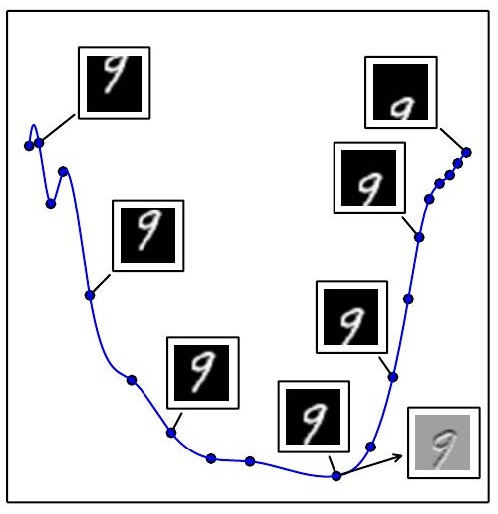
\includegraphics[width=4in]{fig/chap14/14_6.jpg} 
   \caption{超切平面概念示意图。这里我们给出一个784-维空间内的一维流面。我们选取MNIST数据集中的一幅784像素的图像,并沿着竖直方向移动它。这样的一组竖直移动数据定义了沿一维流面方向的坐标,并在图像空间中划出一条曲线。图中给出了在这个流面上的几个点。为了可视效果,我们用PCA把流面投影到了二维空间中。一个n维流面在任一点都有一个n维切面。切面在流面上的该点处完美贴合,并且与该点的表面平行。该切面定义了使得数据保持在流面上的可以移动的方向空间。图中的一维流面有一个单独的切线。我们在图中给出了一个切线示例,以及在图像空间中沿切线移动时所产生的变化。灰色的像素是在移动过程这个不发生变化的点,白色代表颜色变亮,黑色代表颜色加深。}
   \label{fig:14.6}
\end{figure}

所有的自编码器的训练过程是两个限定因素的折衷:

1. 学习一个训练样本$x$的特征表示$h$,使得$x$能够通过解码器从$h$中大致恢复出来。$x$是从训练样本抽取的这个事实使得问题有点儿麻烦,因为这意味着自编码器没有必要对与不在数据生成分布下的输入进行很好的重建。

2. 满足限定或者泛化惩罚。这个可以是结构上限定自编码器的容量的设定,或者是添加到重建误差后的一项泛化项。这些技术通常倾向于对于输入数据不敏感的解决方案。

显然,不管是从输入到输出的复制本身,或者是直接忽略输入,二者任何之一单独出现都没有太大作用。相反,二者同时出现,能够保证方法有效,因为他们迫使隐藏特征表示去捕获能够描述数据生成分布的内在结构。重要的一点就是自编码器可以只去表示重建训练数据所必须的那些变化。如果生成数据的分布本身集中在一个低维流面上,这诱使特征描述仅仅表现这个流面上的一个局部的坐标系统:即只有在$x$附近的与流面相切的变化可以联系到$h = f(x)$的改变上。所以,自编码器学到的从输入空间$x$到表示空间的映射,是一个仅仅对于在流面方向上的变化敏感但对于垂直于流面方向上的变化不敏感的映射。

图\ref{fig:14.7} 给出了一个一维的例子,该图表明通过限定重建函数对于数据点周围扰动的敏感性,我们的自编码器可以重建流面结构。
\begin{figure}[htbp] %  figure placement: here, top, bottom, or page
   \centering
   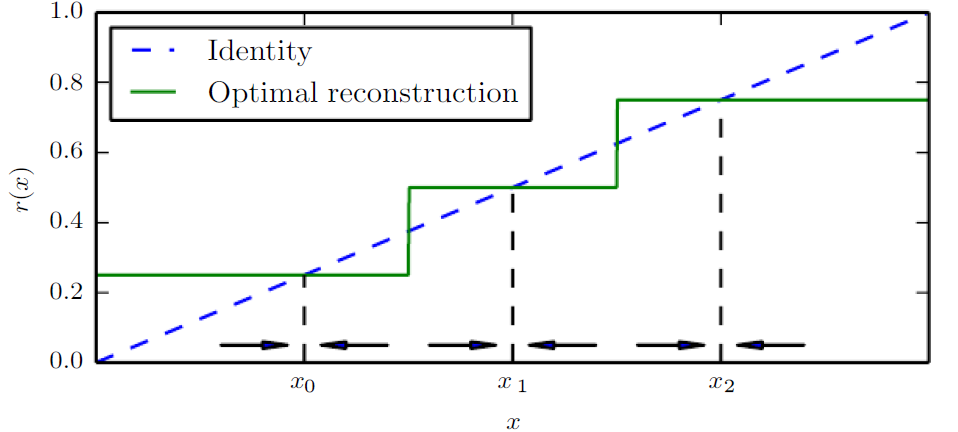
\includegraphics[width=4in]{fig/chap14/14_7.png} 
   \caption{如果自编码器学习到了一个能够对在数据点周围的扰动具有不变性的重建方程,则其学习到了数据本身的流行结构。图中给出的是0-维流面的流行结构。虚线表示用以重建的恒等函数。最有重建函数在有数据的地方同恒等函数重合。底部的箭头表示重建误差向量$r(x)-x$,在输入空间,这些箭头总是指向其最近的“流面”(在一维的情况下,是一个孤立点)。降噪自编码器直接设法使重建函数$r(x)$的偏导数在数据点周围尽量小。收缩自编码器对于编码器进行了同样的操作。尽管$r(x)$的导数在数据点周围尽量小,在不同数据点之间,它可以变得很大。数据点之间的空间同流面之间的区域直接相关,在这些地方,重建函数的导数必须很大,才能将被破坏的点重新映射回流面上。}
   \label{fig:14.7}
\end{figure}

为了更好的理解为什么自编码器可以进行流行学习,我们有必要将其与其他方法进行比较 。对于流行的特性最常用的研究方法是点在流面上或者流面附近的\emph{特征表示}。对于某个样本的特征表示也被称作其嵌入。特征表示通常用一个低维的向量来表示,即比作为一个低维子集存在的流面的原始外部空间的维数要低。一些算法直接对每一个训练样本学习一个嵌入表示(如下面导论到的非参数流行学习方法),与此同时,其他的一些方法则设法学习到一个更为通用的映射,该映射将周围空间(输入空间)映射到嵌入空间。有时这种映射被叫做自编码器或者表示方程式。 

流行学习通常关注于非监督学习的方法来得到这些流面。早期的大部分学习流面的研究集中在基于最近邻图模型的非参数方法上。在图模型中,每个样本表示为一个节点,并通过边将最近邻的样本连接起来。如图\ref{fig:14.8}所示,这些方法将每个节点表示为切平面,这些切平面描述了样本同其邻域样本的变化方向。
\begin{figure}[htbp] %  figure placement: here, top, bottom, or page
   \centering
   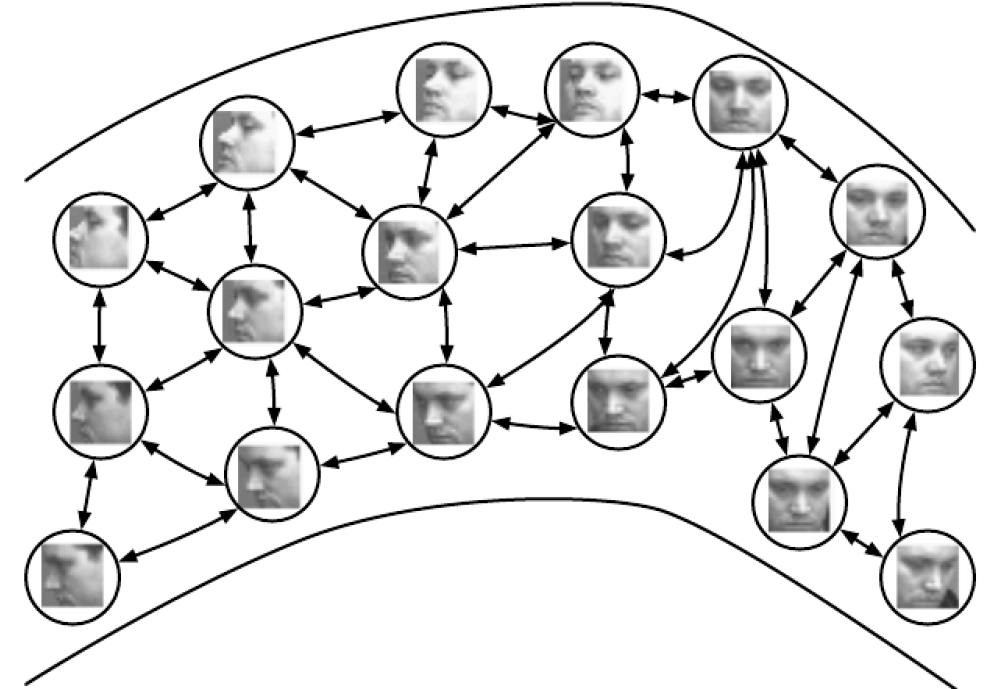
\includegraphics[width=4in]{fig/chap14/14_8.png} 
   \caption{非参数流行学习方法构建了一个最近邻图模型,其中,节点表示训练样本,有向边表明最近邻关系。如此,通过各种不同的方法可以得到切平面以及与其相对应的邻域图模型,此外,还有一个将每一个样本同一个实值向量或嵌入对应的坐标系统。如此我们可以通过一定的改动使特征表示适应新的样本。只要样本数量足够大能够覆盖流面的弯曲与褶皱,这些方法都可以很好的工作。图片来源为QMUL多视人脸数据库。}
   \label{fig:14.8}
\end{figure}

我们之后可通过优化算法或者求解线性系统来获取一个全局坐标系统。图\ref{fig:14.9}给出了一个流面视如何平铺成大量的局部线性类高斯碎片的(或者叫做圆饼,因为高斯函数在切线方向是平坦的)。
\begin{figure}[htbp] %  figure placement: here, top, bottom, or page
   \centering
   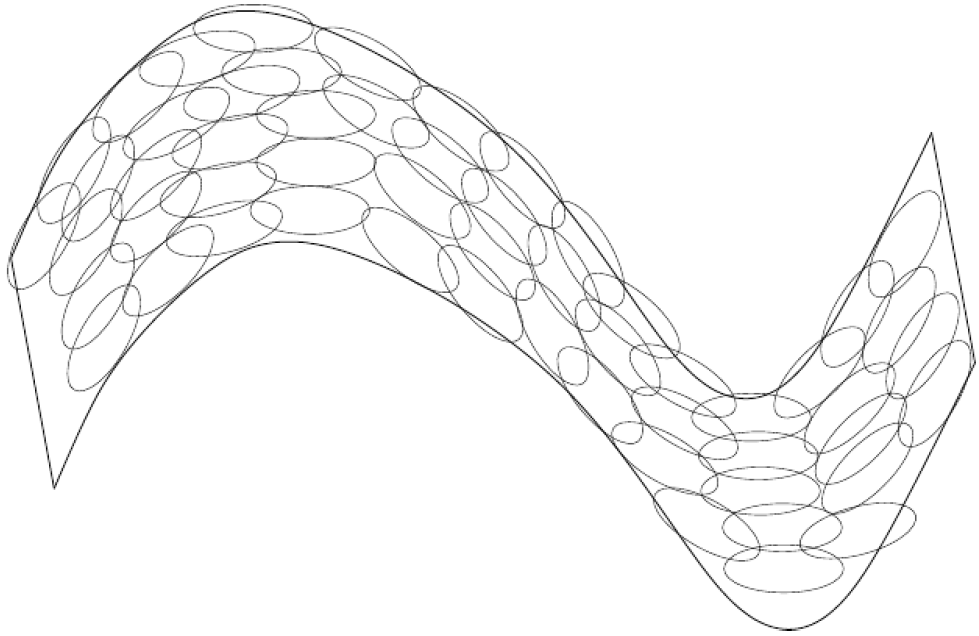
\includegraphics[width=4in]{fig/chap14/14_9.png} 
   \caption{如果切平面(参考图\ref{fig:14.6})在处处都是已知的,则他们可以平铺成一个全局的坐标系统或者密度方程。每一个局部分块都可以被看成是一个局部的欧氏坐标系统或者局部扁平高斯或者圆盘,他们在垂直于圆盘的方向变化很小,在定义圆盘坐标系统的方向上变化很大。这样的一些高斯函数组合成了在流面高斯窗算法或者其基于非局部神经网络的变种中的一个预测密度函数。}
   \label{fig:14.9}
\end{figure}

但是,用这些局部非参数的方法在进行流行学习的时候有一个基本的难题:如果流面本身非常不平整(有许多峰值、低谷、褶皱),我们可能需要大量的样本来覆盖这些变量,从而降低了对未知样本的泛化能力。事实上,这些方法仅仅能够通过邻域信息的插值来泛化流面的形状。不幸的是,在人工智能问题中涉及到的流行往往具有非常复杂的结构,很难从局部插值中获取所有信息。比如说图\ref{fig:14.6}中的通过平移变换产生的流面,如果我们仅仅观察输入向量的一个坐标$x_i$的话,当图像移动时,我们可以看到,每当图像在遇到灰度的峰值或者低谷的时候,我们的坐标就会遇到一个峰值或者低谷。换言之,待处理图像的灰度明暗的复杂度决定了对于像进行简单的平移操作产生的流面的复杂度。这些促使了通过分布式描述和深度学习进行流行结构学习的需求。